% xcolor and define colors -------------------------
\usepackage{xcolor}

% https://www.viget.com/articles/color-contrast/
\definecolor{purple}{HTML}{5601A4}
\definecolor{navy}{HTML}{0D3D56}
\definecolor{ruby}{HTML}{9a2515}
\definecolor{alice}{HTML}{107895}
\definecolor{daisy}{HTML}{EBC944}
\definecolor{coral}{HTML}{F26D21}
\definecolor{kelly}{HTML}{829356}
\definecolor{cranberry}{HTML}{E64173}
\definecolor{jet}{HTML}{131516}
\definecolor{asher}{HTML}{555F61}
\definecolor{slate}{HTML}{314F4F}

% Mixtape Sessions
\definecolor{picton-blue}{HTML}{00b7ff}
\definecolor{violet-red}{HTML}{ff3881}
\definecolor{sun}{HTML}{ffaf18}
\definecolor{electric-violet}{HTML}{871EFF}

\newcommand\pictonBlue[1]{{\color{picton-blue}#1}}
\newcommand\sun[1]{{\color{sun}#1}}
\newcommand\electricViolet[1]{{\color{electric-violet}#1}}
\newcommand\violetRed[1]{{\color{violet-red}#1}}

\newcommand\bgPictonBlue[1]{{\colorbox{picton-blue!20!white}{#1}}}
\newcommand\bgSun[1]{{\colorbox{sun!20!white}{#1}}}
\newcommand\bgElectricViolet[1]{{\colorbox{electric-violet!20!white}{#1}}}
\newcommand\bgVioletRed[1]{{\colorbox{violet-red!20!white}{#1}}}

\def\code#1{\texttt{#1}}

% Main theme colors
\definecolor{accent}{HTML}{00b7ff}
\definecolor{accent2}{HTML}{871EFF}
\definecolor{gray100}{HTML}{f3f4f6}
\definecolor{gray800}{HTML}{1F292D}


% Beamer Options -------------------------------------

% Background
\setbeamercolor{background canvas}{bg = white}

% Change text margins
\setbeamersize{text margin left = 15pt, text margin right = 15pt} 

% \alert
\setbeamercolor{alerted text}{fg = accent2}

% Frame title
\setbeamercolor{frametitle}{bg = white, fg = jet}
\setbeamercolor{framesubtitle}{bg = white, fg = accent}
\setbeamerfont{framesubtitle}{size = \small, shape = \itshape}

% Block
\setbeamercolor{block title}{fg = white, bg = accent2}
\setbeamercolor{block body}{fg = gray800, bg = gray100}

% Title page
\setbeamercolor{title}{fg = gray800}
\setbeamercolor{subtitle}{fg = accent}

%% Custom \maketitle and \titlepage
\setbeamertemplate{title page}
{
    %\begin{centering}
        \vspace{20mm}
        {\Large \usebeamerfont{title}\usebeamercolor[fg]{title}\inserttitle}\\
        {\large \itshape \usebeamerfont{subtitle}\usebeamercolor[fg]{subtitle}\insertsubtitle}\\ \vspace{10mm}
        {\insertauthor}\\
        {\color{asher}\small{\insertdate}}\\
    %\end{centering}
}

% Table of Contents
\setbeamercolor{section in toc}{fg = accent!70!jet}
\setbeamercolor{subsection in toc}{fg = jet}

% Button 
\setbeamercolor{button}{bg = accent}

% Remove navigation symbols
\setbeamertemplate{navigation symbols}{}

% Table and Figure captions
\setbeamercolor{caption}{fg=jet!70!white}
\setbeamercolor{caption name}{fg=jet}
\setbeamerfont{caption name}{shape = \itshape}

% Bullet points

%% Fix spacing between items
\let\olditemize=\itemize 
\let\endolditemize=\enditemize 
\renewenvironment{itemize}{\vspace{0.25em}\olditemize \itemsep0.25em}{\endolditemize}

%% Fix left-margins
\settowidth{\leftmargini}{\usebeamertemplate{itemize item}}
\addtolength{\leftmargini}{\labelsep}

%% enumerate item color
\setbeamercolor{enumerate item}{fg = accent}
\setbeamerfont{enumerate item}{size = \small}
\setbeamertemplate{enumerate item}{\insertenumlabel.}

%% itemize
\setbeamercolor{itemize item}{fg = accent!70!white}
\setbeamerfont{itemize item}{size = \small}
\setbeamertemplate{itemize item}[circle]

%% right arrow for subitems
\setbeamercolor{itemize subitem}{fg = accent!60!white}
\setbeamerfont{itemize subitem}{size = \small}
\setbeamertemplate{itemize subitem}{$\rightarrow$}

\setbeamertemplate{itemize subsubitem}[square]
\setbeamercolor{itemize subsubitem}{fg = jet}
\setbeamerfont{itemize subsubitem}{size = \small}








% Links ----------------------------------------------

\usepackage{hyperref}
\hypersetup{
  colorlinks = true,
  linkcolor = accent2,
  filecolor = accent2,
  urlcolor = accent2,
  citecolor = accent2,
}


% Line spacing --------------------------------------
\usepackage{setspace}
\setstretch{1.35}


% \begin{columns} -----------------------------------
\usepackage{multicol}


% Fonts ---------------------------------------------
% Beamer Option to use custom fonts
\usefonttheme{professionalfonts}

% \usepackage[utopia, smallerops, varg]{newtxmath}
% \usepackage{utopia}
\usepackage[sfdefault,light]{roboto}

% Small adjustments to text kerning
\usepackage{microtype}



% Remove annoying over-full box warnings -----------
\vfuzz2pt 
\hfuzz2pt


% Table of Contents with Sections
\setbeamerfont{myTOC}{series=\bfseries, size=\Large}
\AtBeginSection[]{
        \frame{
            \frametitle{Roadmap}
            \tableofcontents[current]   
        }
    }


% Tables -------------------------------------------
% Tables too big
% \begin{adjustbox}{width = 1.2\textwidth, center}
\usepackage{adjustbox}
\usepackage{array}
\usepackage{threeparttable, booktabs, adjustbox}
    
% Fix \input with tables
% \input fails when \\ is at end of external .tex file
\makeatletter
\let\input\@@input
\makeatother

% Tables too narrow
% \begin{tabularx}{\linewidth}{cols}
% col-types: X - center, L - left, R -right
% Relative scale: >{\hsize=.8\hsize}X/L/R
\usepackage{tabularx}
\newcolumntype{L}{>{\raggedright\arraybackslash}X}
\newcolumntype{R}{>{\raggedleft\arraybackslash}X}
\newcolumntype{C}{>{\centering\arraybackslash}X}

% Figures

% \imageframe{img_name} -----------------------------
% from https://github.com/mattjetwell/cousteau
\newcommand{\imageframe}[1]{%
    \begin{frame}[plain]
        \begin{tikzpicture}[remember picture, overlay]
            \node[at = (current page.center), xshift = 0cm] (cover) {%
                \includegraphics[keepaspectratio, width=\paperwidth, height=\paperheight]{#1}
            };
        \end{tikzpicture}
    \end{frame}%
}

% subfigures
\usepackage{subfigure}


% Highlight slide -----------------------------------
% \begin{transitionframe} Text \end{transitionframe}
% from paulgp's beamer tips
\newenvironment{transitionframe}{
    \setbeamercolor{background canvas}{bg=accent!40!black}
    \begin{frame}\color{accent!10!white}\LARGE\centering
}{
    \end{frame}
}


% Table Highlighting --------------------------------
% Create top-left and bottom-right markets in tabular cells with a unique matching id and these commands will outline those cells
\usepackage[beamer,customcolors]{hf-tikz}
\usetikzlibrary{calc}
\usetikzlibrary{fit,shapes.misc}

% To set the hypothesis highlighting boxes red.
\newcommand\marktopleft[1]{%
    \tikz[overlay,remember picture] 
        \node (marker-#1-a) at (0,1.5ex) {};%
}
\newcommand\markbottomright[1]{%
    \tikz[overlay,remember picture] 
        \node (marker-#1-b) at (0,0) {};%
    \tikz[accent!80!jet, ultra thick, overlay, remember picture, inner sep=4pt]
        \node[draw, rectangle, fit=(marker-#1-a.center) (marker-#1-b.center)] {};%
}


% DAGS ----------------------------------------------
\usepackage{tikz}
\usetikzlibrary{shapes,decorations,arrows,calc,arrows.meta,fit,positioning}
% Tikz settings optimized for causal graphs.
\tikzset{
    -Latex,auto,node distance =1 cm and 1 cm,semithick,
    state/.style ={ellipse, draw, minimum width = 0.7 cm},
    point/.style = {circle, draw, inner sep=0.04cm,fill,node contents={}},
    bidirected/.style={Latex-Latex,dashed},
    el/.style = {inner sep=2pt, align=left, sloped}
}


% Beamer tricks -------------------------------------
% Make \pause work in align environments
\makeatletter
\renewrobustcmd{\beamer@@pause}[1][]{%
  \unless\ifmeasuring@%
  \ifblank{#1}%
    {\stepcounter{beamerpauses}}%
    {\setcounter{beamerpauses}{#1}}%
  \onslide<\value{beamerpauses}->\relax%
  \fi%
}
\makeatother


%\documentclass[aspectratio=169]{beamer}



% \usepackage{slashbox}
\title{Lecture 2: Maximum Likelihood and Friends}
\author{Chris Conlon }
\institute{NYU Stern }

\newcommand{\fp}{\frame[plain]}

\date{\today}

\begin{document}
\maketitle

\begin{frame}{Introduction}
Consider a linear regression with $\varepsilon_i \mid X_i \sim \mathcal{N}(0,\sigma^2)$
\begin{align*}
Y_{it} &= X_{i}'\beta_i + \varepsilon_{i}
\end{align*}
We've discussed the \alert{least squares estimator}:
\begin{align*}
\widehat{\beta}_{ols} &= \arg \min_{\beta} \sum_{i=1}^N (Y_i - X_i' \beta)^2\\
\widehat{\beta}_{ols} &= (\mathbf{X}'\mathbf{X})^{-1} \mathbf{X}' \mathbf{Y}
\end{align*}
\end{frame}


\begin{frame}{Review: What is a Likelihood?}
Suppose we write down the joint distribution of our data $(y_i,x_i)$ for $i=1,\ldots,n$.
\begin{align*}
\probP(y_1,\ldots,y_n, x_1,\ldots,x_n \mid  \theta)
\end{align*}
If  $(y_i,x_i)$ are I.I.D then we can write this as:
\begin{align*}
 \probP(y_1,\ldots,y_n, x_1,\ldots,x_n \mid \theta) = \prod_{i=1}^N \probP(y_i, x_i \mid \theta) \propto \prod_{i=1}^N \probP(y_i \mid x_i , \theta)=\mathbb{L}( \mathbf{y} \mid \mathbf{x} ,\theta )
\end{align*}
We call this $\mathbb{L}( \mathbf{y}\mid \mathbf{x} ,\theta )$ the \alert{likelihood} of the observed data.
\end{frame}




\begin{frame}{MLE: Example}
If we know the distribution of $\varepsilon_i$ we can construct a \alert{maximum likelihood estimator}
\begin{align*}
(\widehat{\beta}_{MLE},\widehat{\sigma}^2_{MLE}) &= \arg \min_{\beta,\sigma^2} \mathbb{L}(\beta,\sigma^2)
\end{align*}
Where 
\begin{align*} 
\mathbb{L}(\beta,\sigma^2) &= \prod_{i=1}^N \probP(y_i \mid x_i,\beta,\sigma^2) \\
                  &= \prod_{i=1}^N \frac{1}{\sqrt{2 \pi \sigma^2}} \exp \left[-\frac{1}{2\sigma^2}(Y_i - X_i' \beta)^2 \right]\\
\ell(\beta,\sigma^2) &= \sum_{i=1}^N -\frac{1}{2} \ln (2 \pi \sigma^2) - \frac{1}{2 \sigma^2} \sum_{i=1}^N(Y_i - X_i' \beta)^2
\end{align*}
\end{frame}

\begin{frame}{MLE: FOC's}
Take the FOC's of: 
$\ell(\beta,\sigma^2) = -\frac{N}{2} \ln (2 \pi \sigma^2) - \frac{1}{2 \sigma^2} \sum_{i=1}^N(Y_i - X_i' \beta)^2
$:
\begin{align*} 
\frac{ \partial \ell(\beta,\sigma^2) }{\partial \beta}&= \frac{1}{ \sigma^2}\sum_{i=1}^N(Y_i - X_i' \beta) = 0 \rightarrow \widehat{\beta}_{MLE}= \widehat{\beta}_{OLS}\\ 
\frac{ \partial \ell(\beta,\sigma^2) }{\partial \sigma^2}&= -N \frac{1}{2 \sigma^2}  -  \frac{1}{2 \sigma^4} \sum_{i=1}^N(Y_i - X_i' \beta)^2 = 0 \\
\sigma^2_{MLE} &= \frac{1}{N} \sum_{i=1}^N (Y_i - X_i' \beta)^2
\end{align*}
Note: the unbiased estimator uses $\frac{1}{N-K-1}$.
\end{frame}

\begin{frame}{MLE: General Case}
\begin{enumerate}
\item Start with the \alert{joint density of the data} $Z_1,\ldots,Z_N$ with density $f_Z(z,\theta)$
\item Construct the likelhood function of the sample $z_1,\ldots,z_n$
\begin{align*}
\mathbb{L}(\mathbf{z} \mid  \theta) = \prod_{i=1}^N f_Z(z_i,\theta)
\end{align*}
\item Construct the \alert{log likelihood} (this has the same $\arg \max$)
\begin{align*}
\ell(\mathbf{z} \mid \theta) = \sum_{i=1}^N \ln f_Z(z_i,\theta)
\end{align*}
\item Take the FOC's to find $\widehat{\theta}_{MLE}$
\begin{align*}
\theta : \frac{\partial \ell(\theta)}{\partial \theta} =0
\end{align*}
\end{enumerate}
\end{frame}

\begin{frame}{MLE in Detail}
Basic Setup: we know $F(z \mid \theta_0)$ but not $\theta_0$. We know $\theta_0 \in \Theta \subset \mathbb{R}^K$.
\begin{itemize}
\item Begin with a sample of $z_i$ from $i=1,\ldots,N$ which are I.I.D. with CDF $F(z|\theta_0)$.
\item The MLE chooses
\begin{align*}
\widehat{\theta}_{MLE} = \arg \max_{\theta} \ell(\theta) = \arg \max_{\theta} \sum_{i=1}^N \ln f_Z(z_i,\theta)
\end{align*}
\end{itemize}
\end{frame}


\begin{frame}{MLE: Technical Details}
\begin{enumerate}
\item Consistency. When is it true that for $\epsilon>0$?
\begin{align*}
\lim _ { N \rightarrow \infty } \probP \left( \left\| \hat { \theta } _ { m l e } - \theta _ { 0 } \right\| > \varepsilon \right) = 0
\end{align*}
\item Asymptotic Normality. What else do we need to show?
\begin{align*}
\sqrt { N } \left( \hat { \theta } _ { m l e } - \theta _ { 0 } \right) \stackrel { d } { \longrightarrow } \mathcal { N } \left( 0 , - \left[ E \frac { \partial ^ { 2 } } { \partial \theta \partial \theta ^ { \prime } } \left( Z _ { i } , \theta _ { 0 } \right) \right] ^ { - 1 } \right)
\end{align*}
\item Optimization. How to we obtain $\widehat{\theta}_{MLE}$ anyway?
\end{enumerate}
\end{frame}


\begin{frame}{MLE: Example \# 1}
\begin{itemize}
\item $Z_i \sim \mathcal{N}(\theta_0,1)$ and $\Theta = (-\infty,\infty)$. In this case:
\begin{align*}
\ell ( \theta ) = - N \cdot \ln ( 2 \pi ) - \sum _ { i = 1 } ^ { N } \left( z _ { i } - \theta \right) ^ { 2 } / 2
\end{align*}
\item MLE is $\widehat{\theta}_{MLE}=\overline{z}$ which is consistent for $\theta_0 = \E[Z_i]$
\item Asymptotic distribution is $\sqrt{N} ( \overline{z}-\theta_0) \sim \mathcal{N}(0,1)$.
\item Calculating mean is easy!
\end{itemize}
\end{frame}




\begin{frame}{MLE: Example \# 2}
\begin{itemize}
\item $Z_i = (Y_i, X_i)$---   $X_i$ has finite mean and variance (but arbitrary distribution)
\item $(Y_i | X_i  =x) \sim  \mathcal{N}(x' \beta_0, \sigma_0^2)$
\begin{align*}
\widehat{\beta}_{MLE} &= (X'X)^{-1} X'Y\\
\widehat{\sigma}^2_{MLE} &= \frac{1}{N} \sum (y_i - x_i \widehat{\beta}_{MLE})^2
\end{align*}
\item We already have shown consistency and AN for linear regression with normally distributed errors...
\end{itemize}
\end{frame}


\begin{frame}{MLE: Example \# 3}
\begin{itemize}
\item $Z_i = (Y_i, X_i)$---   $X_i$ has finite mean and variance (but arbitrary distribution)
\item $\probP(Y_i=1 | X_i =x) =  \frac{e^{x' \theta_0}}{1+ e^{x'\theta_0}}$
\item Solution is the \alert{logit} model.
\item No simple MLE solution, establishing properties is not obvious...
\end{itemize}
\end{frame}

\begin{frame}{Jensen's Inequality}
\begin{columns}[T]
\begin{column}{.4\textwidth}
Let $\phi(z)$ be a convex function.\\ 
\vspace{2cm}
Then $\E[\phi(Z)] \geq \phi(\E [Z])$, with equality only in the case of a linear function.
\end{column}
\hfill
\begin{column}{.6\textwidth}
\begin{center}
 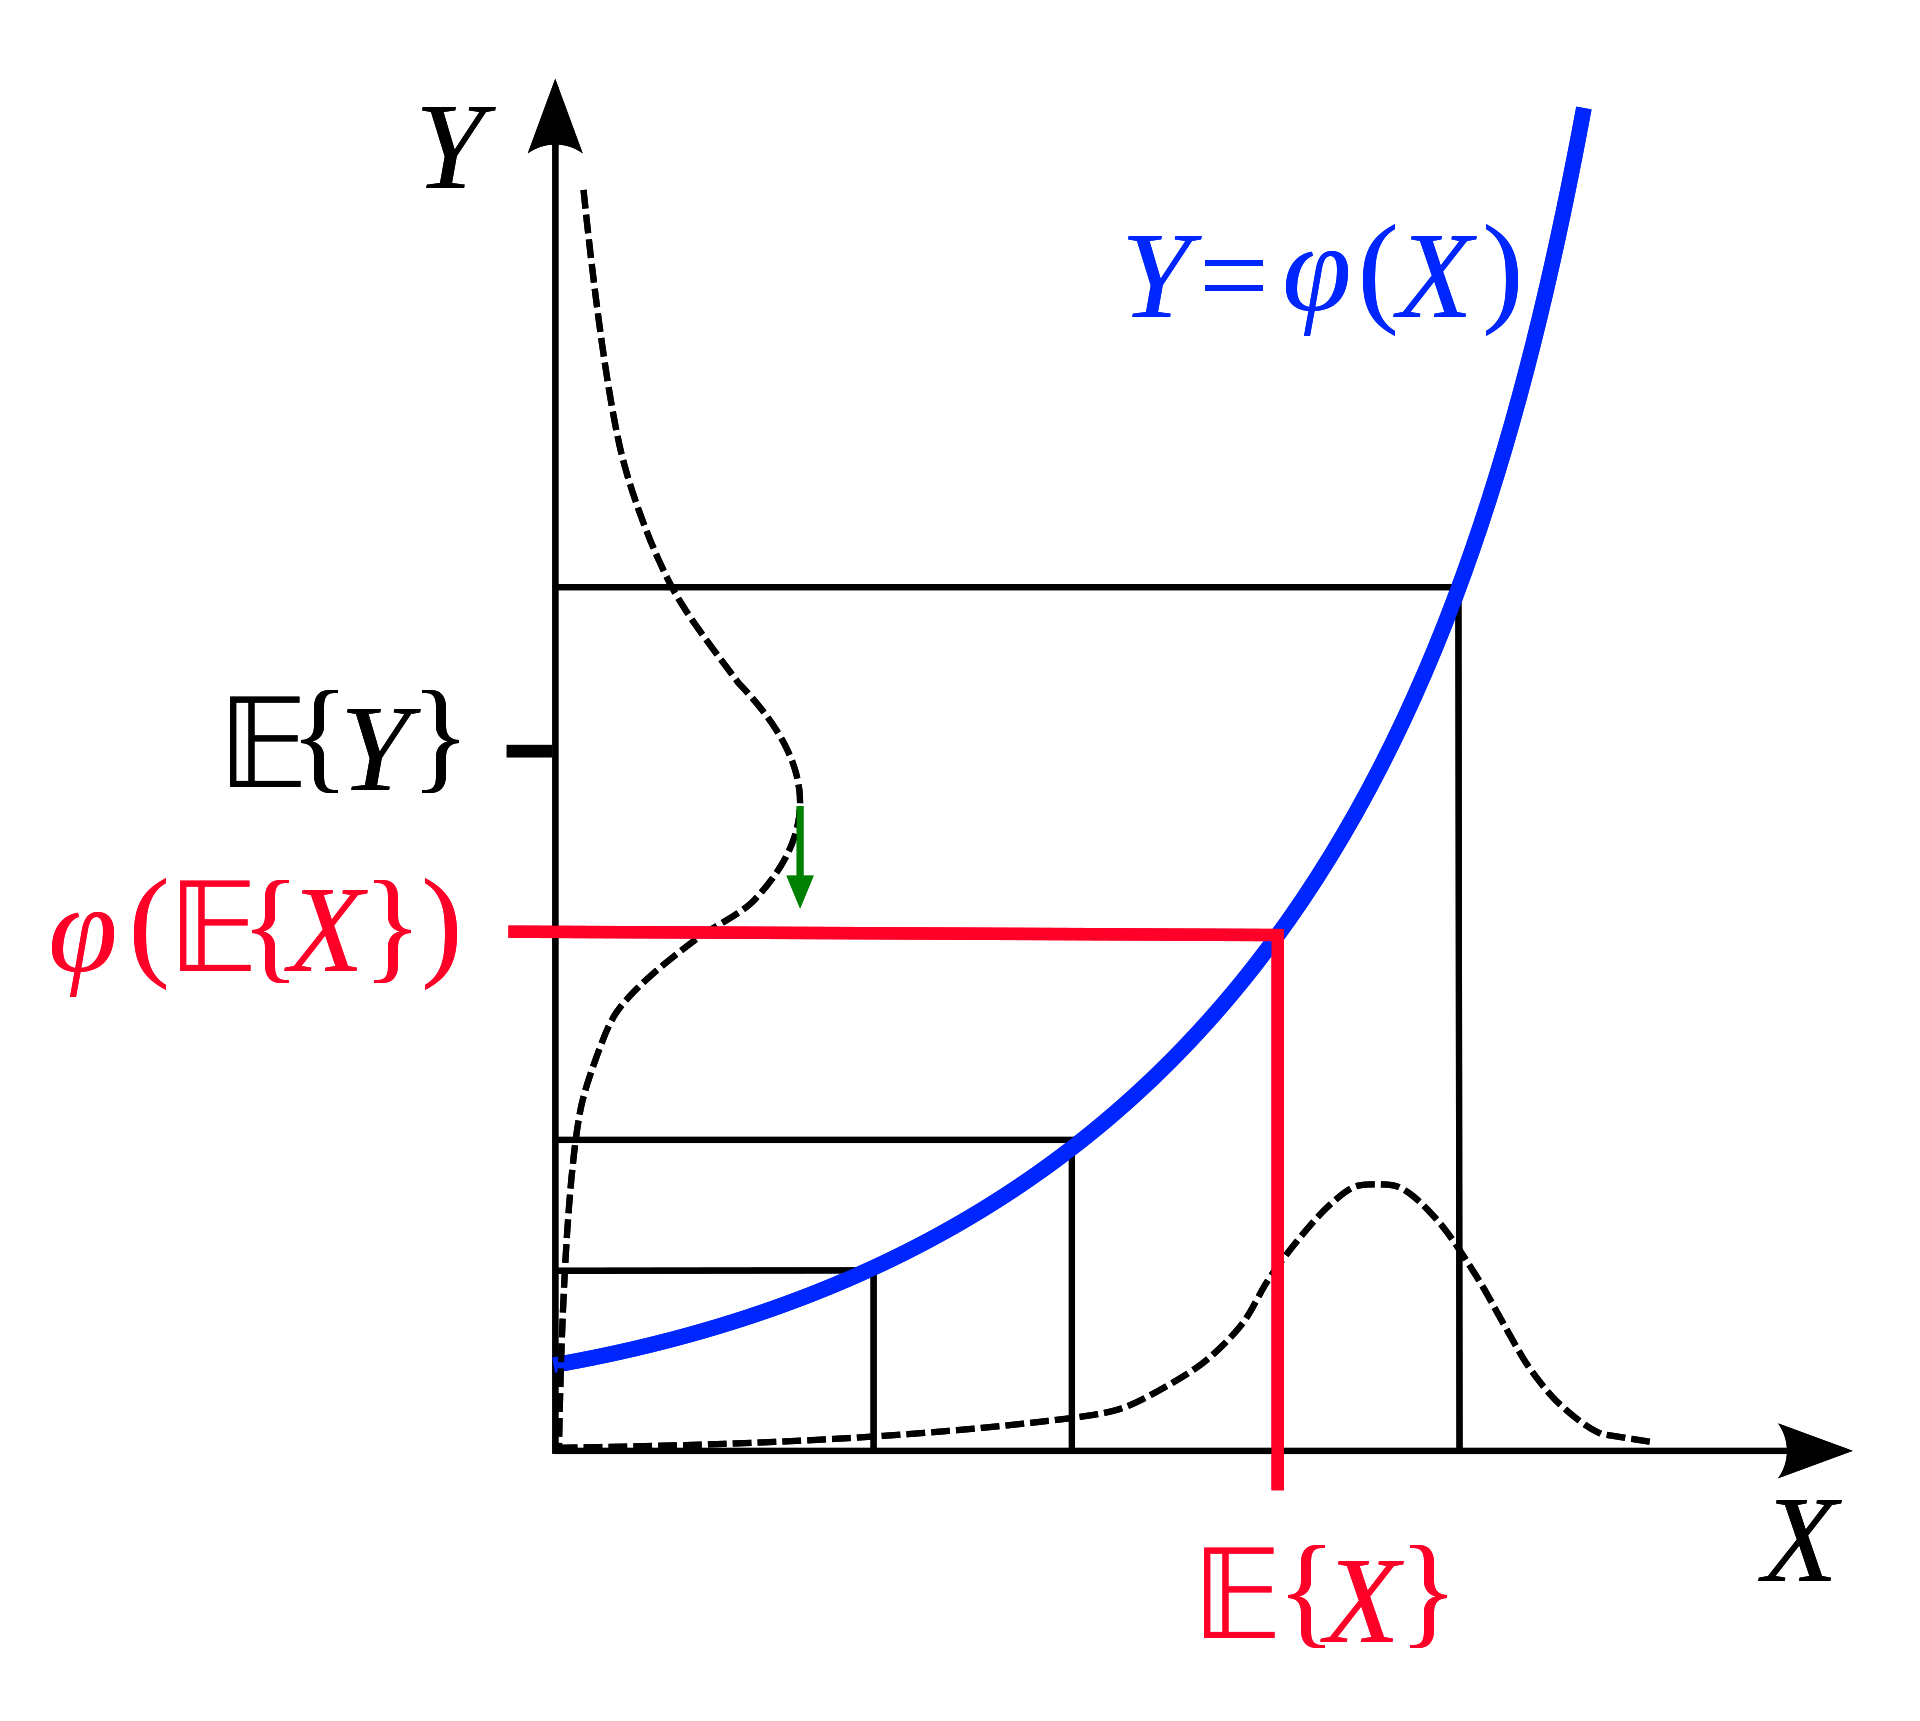
\includegraphics[width=0.9\textwidth]{resources/jensen.png}
\end{center}
\end{column}
\end{columns}



\end{frame}

\begin{frame}{More Technical Details}
Define $Y$ as the ratio of the density at $\theta$ to the density at the true value $\theta_0$ both evaluated at $Z$
\begin{align*}
Y = \frac{f_Z(Z;\theta)}{f_Z(Z;\theta_0)}
\end{align*}
\vspace{-0.5cm}
\begin{itemize}
\item Let $g(a) = -\ln(a)$ so that $g'(a) = \frac{-1}{a}$ and $g''(a) =\frac{1}{a^2}$.
\item Then by \alert{Jensen's Inequality} $\mathbb{E}[- \ln Y] \geq - \ln \mathbb{E}[Y]$.
\item This gives us
\begin{align*}
\mathbb { E }_z \left[ - \ln \left( \frac { f _ { Z } ( Z ; \theta ) } { f _ { Z } \left( Z ; \theta _ { 0 } \right) } \right) \right] \geq - \ln \left( \mathbb { E }_z \left[ \frac { f _ { Z } ( Z ; \theta ) } { f _ { Z } \left( Z ; \theta _ { 0 } \right) } \right] \right)
\end{align*}
\item The RHS is
\begin{align*}
\mathbb { E }_z \left[ \frac { f _ { Z } ( Z ; \theta ) } { f _ { Z } \left( Z ; \theta _ { 0 } \right) } \right] = \int \frac { f _ { Z } ( z ; \theta ) } { f _ { Z } \left( z ; \theta _ { 0 } \right) } \cdot f _ { Z } \left( z ; \theta _ { 0 } \right) d z = \int f _ { Z } ( z ; \theta ) d z = 1
\end{align*}
\end{itemize}
\end{frame}


\begin{frame}{More Technical Details}
Because $\log(1)=0$ this implies:
\begin{align*}
\mathbb { E }_z \left[ - \ln \left( \frac { f _ { Z } ( Z ; \theta ) } { f _ { Z } \left( Z ; \theta _ { 0 } \right) } \right) \right] \geq 0
\end{align*}
Therefore 
\begin{align*}
- \mathbb { E } \left[ \ln f _ { Z } ( Z ; \theta ) \right] &+ \mathbb { E } \left[ \ln f _ { Z } \left( Z ; \theta _ { 0 } \right) \right] \geq 0\\
\mathbb { E } \left[ \ln f _ { Z } \left( Z ; \theta _ { 0 } \right) \right] &\geq \mathbb { E } \left[ \ln f _ { Z } ( Z ; \theta ) \right]
\end{align*}
\begin{itemize}
\item We maximize the expected value of the log likelihood at the true value of $\theta$!
\item Helpful to work with $\mathbb{E}[\log f(z; \theta)]$ sometimes.
\end{itemize}
\end{frame}


\begin{frame}{Information Matrix Equality}
We can relate the \alert{Fisher Information} to the Hessian of the log-likelihood
\begin{align*}
\mathcal { I } \left( \theta _ { 0 } \right) = - \mathbb { E } \left[ \frac { \partial ^ { 2 } \ln f } { \partial \theta \partial \theta } \left( z ; \theta _ { 0 } \right) \right] 
= \mathbb { E } \left[ \frac { \partial \ln f } { \partial \theta } \left( z ; \theta _ { 0 } \right) \times \frac { \partial \ln f } { \partial \theta  } \left( z ; \theta _ { 0 } \right)' \right]
\end{align*}
\begin{itemize}
    \item This is sometimes known as the \alert{outer product of scores}.
    \item This matrix is \alert{negative definite}
    \item Recall that $ \mathbb { E } \left[ \frac { \partial \ln f } { \partial \theta } \left( z ; \theta _ { 0 } \right) \right]\approx 0$ at the maximum
\end{itemize}
\end{frame}


\begin{frame}{Proof}
\begin{align*}
1 = \int _ { z } f _ { Z } ( z ; \theta ) d z \Rightarrow 0 = \frac { \partial } { \partial \theta } \int _ { z } f _ { Z } ( z ; \theta ) d z
\end{align*}
With some regularity conditions
\begin{align*}
0 = \int _ { z } \frac { \partial f _ { Z } } { \partial \theta } ( z ; \theta ) d z = \underbrace{\int _ { z } \frac { \partial \ln f _ { Z } } { \partial \theta } ( z ; \theta ) \cdot f _ { Z } ( z ; \theta ) d z}_{\mathbb { E } \left[ \frac { \partial \ln f _ { Z } } { \partial \theta } \left( z ; \theta _ { 0 } \right) \right]}
\end{align*}

\begin{itemize}
    \item This gives us the FOC we needed.
    \item Can get information identity with another set of derivatives.
    \end{itemize}
\end{frame}


\begin{frame}{The Cramer-Rao Bound}
We can relate the \alert{Fisher Information} to the Hessian of the log-likelihood
\begin{align*}
\mathcal { I } ( \theta ) = - \mathbb { E } \left[ \frac { \partial ^ { 2 } \ln f } { \partial \theta \partial \theta ^ { \prime } } ( Z | \theta ) \right]
\end{align*}
It turns out this provides a bound on the variance
\begin{align*}
\operatorname { Var } ( \hat { \theta } ( Z ) ) \geq \mathcal { I } \left( \theta _ { 0 } \right) ^ { - 1 }
\end{align*}
Because we can't do better than Fisher Information we know that MLE is most efficient estimator!
\end{frame}

\begin{frame}{MLE: Discussion}
Tradeoffs
\begin{itemize}
\item How does this compare to GM Theorem?
\item If MLE is most efficient estimate, why ever use something else?
\end{itemize}
\end{frame}


\begin{frame}{Exponential Example}
\begin{align*}
f _ { Y \mid X } ( y \mid x , \beta _ { 0 } ) =  { e } ^ { x ^ { \prime } \beta _ { 0 } } \exp \left( - y  { e } ^ { x ^ { \prime } \beta _ { 0 } } \right)
\end{align*}
With log likelihood
\begin{align*}
\ell( \beta ) = \sum _ { i = 1 } ^ { N } \ln f _ { Y \mid X } \left( y _ { i } \mid x _ { i } , \beta \right) = \sum _ { i = 1 } ^ { N } X _ { i } ^ { \prime } \beta - y _ { i } \cdot \exp \left( x _ { i } ^ { \prime } \beta \right)
\end{align*}
And Score, Hessian, and Information Matrix:
\begin{align*}
\mathcal { S }_i ( y_i, x_i , \beta ) &= x_i ^ { \prime } \left( 1 - y_i \exp \left( x_i ^ { \prime } \beta \right) \right)\\
\mathcal { H }_i ( y_i , x_i , \beta ) &= - y_i x_i x_i ^ { \prime } \exp \left( x_i ^ { \prime } \beta \right)\\
% WHERE DOES THIS COME FROM
\mathcal { I } \left( \beta _ { 0 } \right) &= \E \left[ Y X X ^ { \prime } \exp \left( X ^ { \prime } \beta _ { 0 } \right) \right] = \E \left[ X X ^ { \prime } \right]
\end{align*}
\end{frame}



\section*{Thanks!}

\end{document}